\documentclass[12pt]{article}
\usepackage[utf8]{inputenc}
\usepackage[T1]{fontenc} % uses T1 fonts (better quality)
\usepackage{helvet} % uses Helvetica
\renewcommand*\familydefault{\sfdefault}
\usepackage[dvipsnames]{xcolor}
\usepackage[margin=1in]{geometry}
\usepackage{nopageno} % no page numbers
\usepackage{graphicx}
\usepackage{subcaption}
\usepackage{tocloft}
\renewcommand{\cftpartleader}{\cftdotfill{\cftdotsep}}
\renewcommand{\cftsecleader}{\cftdotfill{\cftdotsep}}
\graphicspath{ {./graphics/} }
\usepackage{minted} % code syntax
\usemintedstyle{vs}
\usepackage{fancyhdr}
\pagestyle{fancy}
\fancyhf{}
\lhead{Aqua Research}
\rhead{The University of New Mexico}
\rfoot{Page \thepage}
\title{}
\begin{document}
\thispagestyle{empty}
\begin{titlepage}
\vspace*{\fill}
\begin{center}
\setlength{\parskip}{2em}\bfseries
\textsc{\Huge{Aqua Research\\[0.25em]Senior Design Project}}\par
\textsc{\LARGE Controller for K1 Batch Generator}\\[1em]
\textsc{\Large Project Manager: Diego Chavez \& David Kirby\\[0.25em]with John Quinlan}\par
\textsc{\Large The University of New Mexico\\[0.25em]School of Engineering}\\[2cm]
\textsc{\Large Aqua Research, LLC\\5601 Midway Park Place NE\\[0.25em]Albuquerque, NM 87109}\\[2cm]
\textsc{\Large Spring 2020}\\[1.5cm]
\end{center}
\vfill
\begin{figure}[h]
\begin{subfigure}{0.5\textwidth}

\includegraphics[width=0.45\linewidth]{New AR Logo White Background 1.PNG}
\end{subfigure}
\begin{subfigure}{0.7\textwidth}

\includegraphics[width=0.75\linewidth]{new-soe-logo.png}
\end{subfigure}
\end{figure}
\end{titlepage}
\setcounter{figure}{0}
\tableofcontents\vspace{1.5cm}
\addcontentsline{toc}{section}{1\quad List of Figures}
\listoffigures\newpage
\setcounter{section}{+1}
\section{Overview}\setlength{\parskip}{1em}
\subsection{Executive Summary}
We set out to produce a prototype for a user interface controller to be used on the K1 Batch Generator, a product currently under development at Aqua Research, LLC. Our team faced copious issues throughout the course of development, however we were able to accurately and successfully meet each requirement and have produced a working prototype for the company. Five units have already been ordered and will be produced by July 2020.

\noindent The K1 Batch Generator is a very important product under development, and with it underdeveloped countries around the world will be able to access disinfected water through the use of chlorine produced from sodium chloride and electricity. The design of our controller was paramount to the effectiveness of the final product as without reliable hardware and software in our K1 controller, the unit would not be able to automatically monitor production.
 
\noindent Future work will consist of improving upon the efficiency of the code to meet even stricter guidelines. Faulty wiring in the prototyping board also caused one of the primary demuxing logic chips to not have power. Addressing this issue will allow future efforts to connect all of the designed components together for phase two prototyping.

\subsection{Abstract}
Aqua Research, LLC has developed systems that use electrolysis to create chlorine from basic table salt. This chlorine can then be used as a disinfectant to create potable water. With applications ranging from emergency response situations, third-world countries, and the military, it was imperative that end-users be able to remotely monitor and maintain these systems during less than ideal conditions. As most of the practical uses for the disinfectant systems are in difficult-to-access areas, it was also beneficial for Aqua Research to be able to troubleshoot these control systems while off-site.

\noindent For example, the team at Aqua Research have done tremendous work in Haiti following devastating earthquakes in 2010 and 2018. Being able to analyze these water treatment systems in Haiti remotely would greatly increase Aqua Research’s presence there and its ability to help more people.

\noindent The senior design group of Aqua Research set out to create a sensor system using cost-effective components that could read data from the disinfectant tanks, detect faults, and report these findings.

\noindent The device needed to be multilingual as it will be used in a variety of countries and situations; it needed to be able to recover from power loss without losing state; and it needed to be able to communicate via long-range telecommunications.

\section{Problem Description}
Aqua Research, LLC develops innovative water treatment technologies that meet the extreme needs within developing countries and provides sustainable water purification to outdoor enthusiasts, travelers, emergency preppers, first responders, Peace Corps, and the military. Their expertise primarily resides in electrolytic technologies that produce disinfectants from salt to a variety of water filtration devices.

\noindent The use cases for these water treatment technologies call for the system to be remotely monitored. Our goal in this project was to design a communication system that could relay alerts via cellular GSM (global system for mobile communications) and to be able to display alert codes locally on an attached LCD and in a variety of languages. The device must be able to:
\begin{enumerate}
    \item monitor digital and analog I/O of the disinfectant controller, including switch levels, indicator LEDs, and current/voltage levels,
    \item have a simple and universal user interface and adaptable to a variety of languages,
    \item recover from power loss without losing state,
    \item communicate via GSM telecommunications, and
    \item be cost-efficient as these devices are primarily meant for low-income and disaster areas.
\end{enumerate}
\noindent A 2015 Senior Design group had previously attempted to create the K1 controller; however, they were only successful in designing a test bench, no working prototype. We took this as a challenge and set out formulating a strategy.
\begin{figure}[h!]
    \centering
    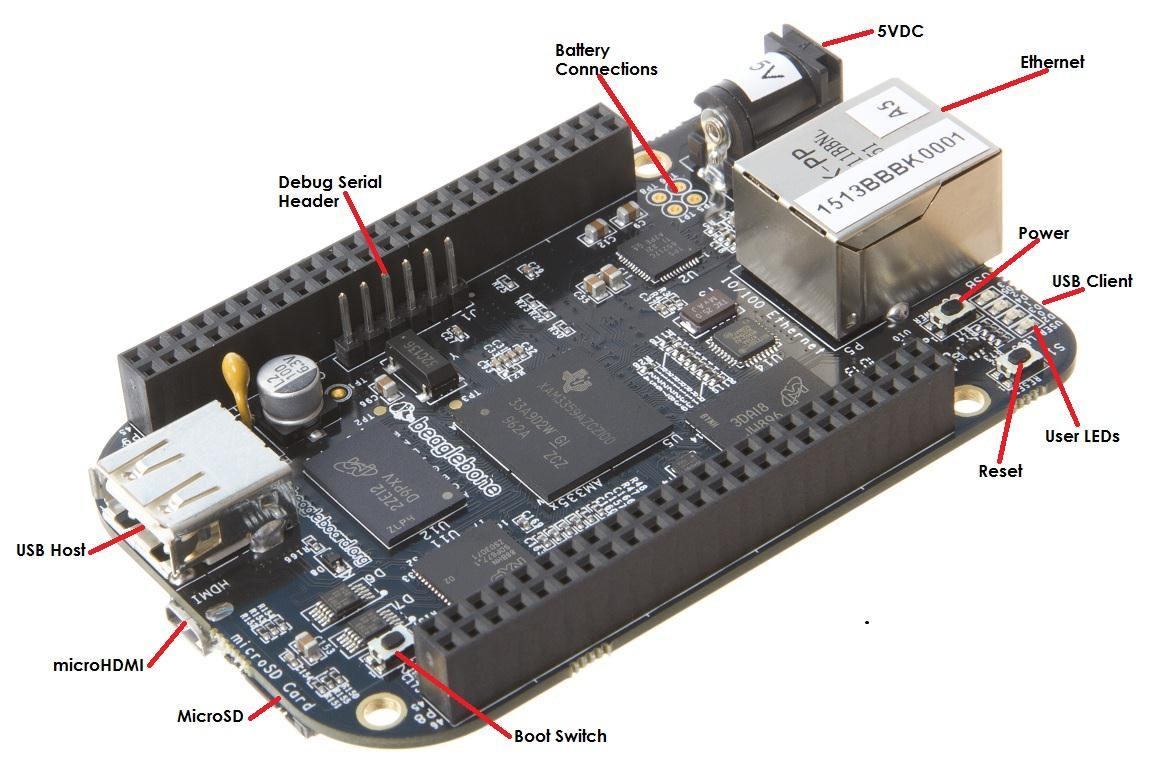
\includegraphics[width=0.55\textwidth]{BBB-Diagram.jpg}
    \caption{Beagle-Bone Black.}
    \label{fig:BeagleBoneBlack}
\end{figure}
\section{Progress Toward a Solution}
The Aqua Research Senior Design Group went through many iterations of control boards. After analyzing a past group’s prototype using a Beagle-Bone Black (Figure~\ref{fig:BeagleBoneBlack}, page~\pageref{fig:BeagleBoneBlack}), we determined that we wanted to build a prototype with a newer microcontroller. We looked for one with smaller footprint and lower power consumption. Initially considering a Raspberry Pi configuration, the Raspberry Pi Zero W met our requirements for lower profile, built-in wireless, and was inexpensive. The Raspberry Pi 4 was powerful and had Wi-Fi support; however, neither of the Raspberry Pis natively supported analog inputs.

\noindent After discussing this with our Technical Mentor\footnote{Tim Cushman, Aqua Research, LLC}, it was suggested that we use the Arduino Nano as it was already implemented in other Aqua Research projects. While the last-minute change was a challenge, it proved to be the best option as it was not only less expensive but also fulfilled every requirement.
\begin{figure}[h!]
    \centering
    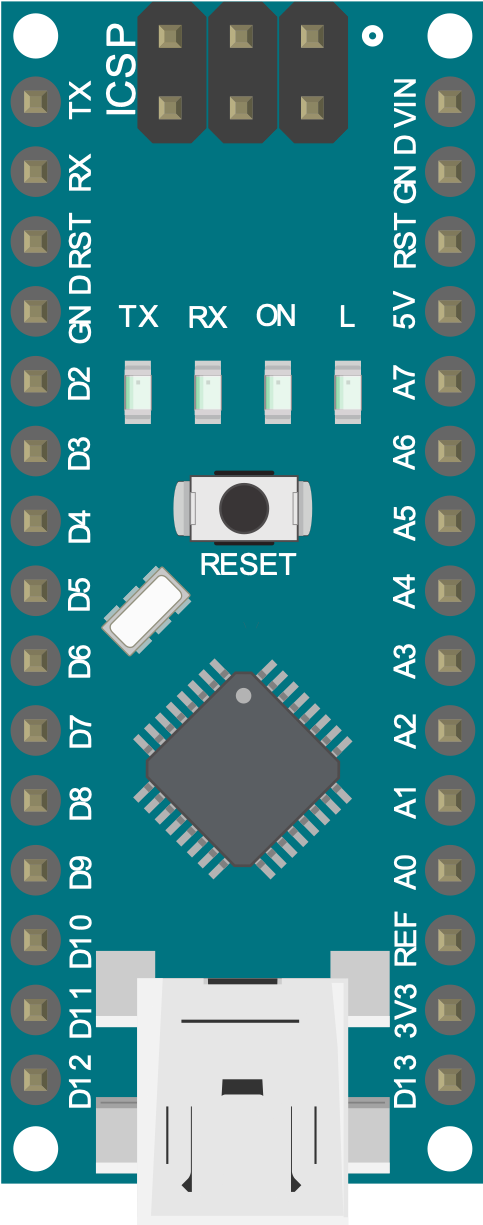
\includegraphics[width=0.15\textwidth, angle=270]{nano.png}
    \caption{Arduino Nano.}
    \label{fig:ArduinoNano}
\end{figure}

\noindent After spending the first semester understanding and setting up the sensor board used to monitor the disinfectant tank, we began the second semester creating pinout mappings for the microcontroller. Using the Arduino IDE, we broke our project down into three main modules: memory, GSM, and display.

\noindent We were successful in configuring two non-volatile memory units to be used as language databases for our sensor display. Each ferroelectric RAM, or FRAM, can store up to 32 kilobytes of information. FRAMs are comparable to dynamic random-access memory but with a ferroelectric layer instead of dielectric layer. This makes it non-volatile but with the responsiveness of dynamic RAM. The FRAMs use I2C interface and one of the challenges of this setup was in connecting the components together so that we could read and write to the modules individually. We accomplished changing FRAM addresses by driving specific individual pins high.

\noindent Next, we focused on the communication network. We opted for using a GSM (global system for mobile communication) breakout board, and though there were issues with the pins used, we were adamant to solve it. There were issues on which pins to use and how to address the board. The module is a Quad-band GSM/GPRS solution and can transmit SMS and data with low power consumption. Once we were successful in wiring it to the Arduino, we activated a SIM card and programmed the board to transmit using case statements based on our test scenarios.

\noindent Finally, our last requirement was to display the sensor feedback using a $4\times20$ LCD screen. This was also connected via I2C and allowed us to display user instructions and alerts. Together, these three modules allowed us to successfully complete our project, providing Aqua Research with a prototype which is now being implemented.
\begin{figure}[h!]
    \centering
    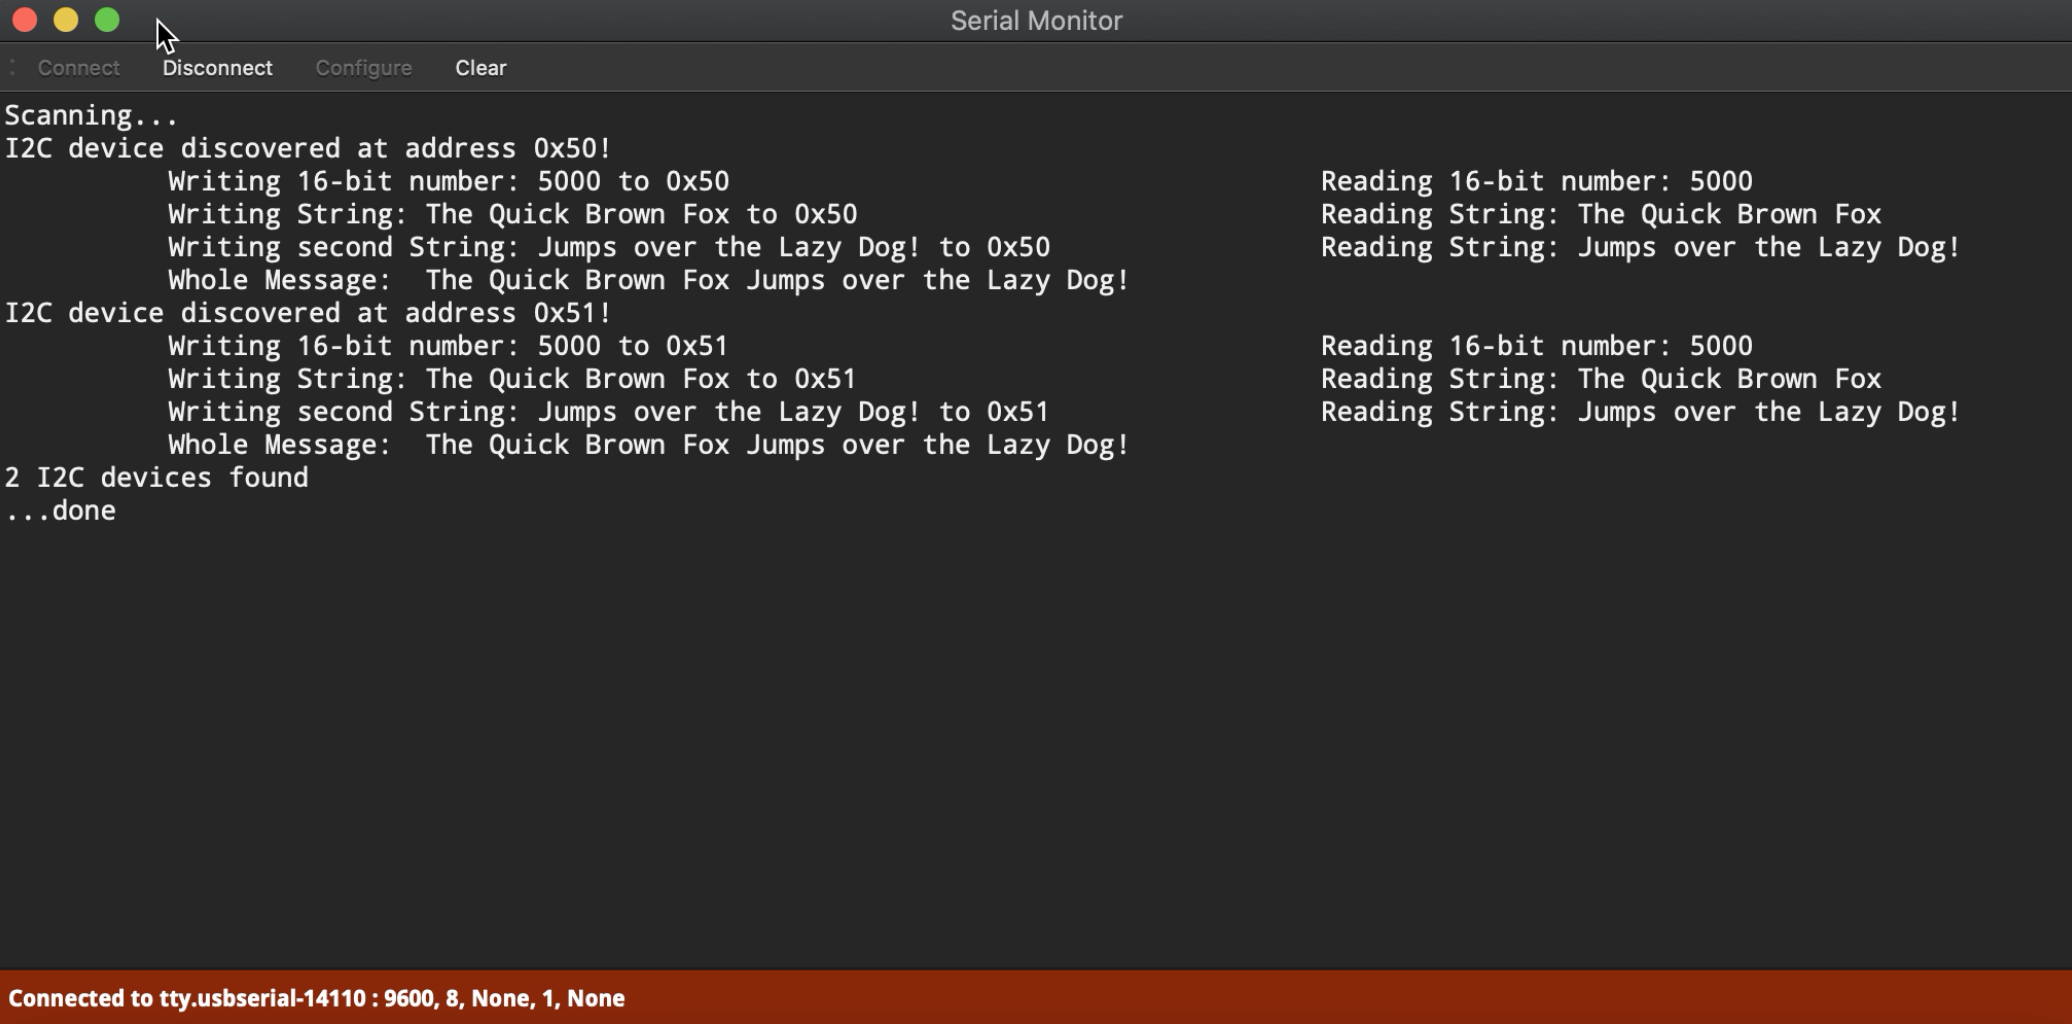
\includegraphics[width=0.85\textwidth]{Screenshot.png}
    \caption{I2C Demonstration.}
    \label{fig:I2Cdemo}
\end{figure}
\section{Constraints}
The Arduino Nano (Figure~\ref{fig:ArduinoNano}, page~\pageref{fig:ArduinoNano}) uses the ATmega328 chipset and has 32 KB of memory with 2 KB used for the bootloader. The ATmega328 has 2 KB of SRAM and 1 KB of EEPROM. Each of the 14 digital pins on the Nano can be used as an input or output and operate at 5 volts. The Nano has 8 analog inputs, each of which provide 10 bits of resolution (i.e. 1024 different values). Finally, the Nano has I2C which we used extensively for this project.
\section{Budget}
\section{Work Schedule}
\section{Personnel Interactions}
\subsection{Teamwork}
\subsection{Mentorship}
\section{Summary \& Conclusions}
Spring 2020 was quite a semester for everyone across the globe and our Aqua Research Senior Design Group was no exception. The University of New Mexico shutting down all in-person operations, and the state and federal governments implementing social-distancing protocols meant working together on the project was quite a challenge.

\noindent While it is undeniable that the coronavirus had an impact on our Senior Design project, we attempted to stay focused and driven in our pursuit of creating a communication system for Aqua Research’s water disinfectant tanks. We stayed in constant contact via text, email, teleconferencing software, and UNM’s LoboGit repository to collaborate on the code for the project. This allowed us to make considerable progress given the circumstances, all while adhering to the stay-at-home orders.

\section{Discussion}
Future opportunities for this project could include programming different databases to the FRAM modules so that they may be hot-swapped as needed. 

\noindent We would also like to see the code optimized as even with the extended modules we were still running low on programmable memory.

\noindent Finally, we would like to extend the code and board to be able to accept various telecommunication modules. Not everywhere uses the same network and bands, and it would be ideal to support as many areas as possible. Perhaps the GSM module could be swapped out depending upon the location where the device will be used.
\section{Acknowledgements}
We are grateful for our sponsors\footnote{Rodney Herrington, Sponsor; Tim Cushman, Technical Mentor, Lois Warren, Technical Mentor} and faculty\footnote{Dr. Ramiro Jordan, Lead Instructor; Dr. Ganesh Balakrishnan, Assistant Instructor; Bradley Evans, Teaching Assistant} in helping us achieve our goals for this project. On behalf of the Aqua Research Senior Design Group, thank you!
\section{References}
\begin{itemize}
    \item Rodney Herrington, “2015 Requirements Document”,
    \item Tim Cushman, “K1 System Schematic”, Document: \texttt{K1K2SYS.SCH}
    \item Tim Cushman, “K1 K2 Disinfection Controller”, Document: \texttt{K1K2.SCH}
    \item Tim Cushman, “K1-K2 Controller Wiring Diagram”, Rev. 3/2020
    \item Tim Cushman, “Ox Tank Floats”, Document: \texttt{K2FLOAT.SCH}
    \item Tim Cushman, “Brine and Oxidant Generator Floats”, Document: \texttt{K1FLOAT.SCH}
    \item Tim Cushman, “K1 K2 Drivers”, Document: \texttt{K1K2DRV.SCH}
    \item Arduino Resources, Address: https://www.arduino.cc
    \item Adafruit I2C FRAM Resources, Address: https://www.adafruit.com/product/1895
\end{itemize}

\newpage
\section{Source Code}
\subsection{final.ino}
\inputminted[frame=lines, linenos, fontsize=\footnotesize]{cpp}{code/final.ino}\newpage
\subsection{I2C\_string.cpp}
\inputminted[frame=lines, linenos, fontsize=\footnotesize]{cpp}{code/I2C_string.cpp}\newpage
\subsection{I2C\_string.h}
\inputminted[frame=lines, linenos, fontsize=\footnotesize]{cpp}{code/I2C_string.h}

\end{document}